\section{Running Example}
\label{sec:example}

%\begin{figure*}
%\begin{center}
%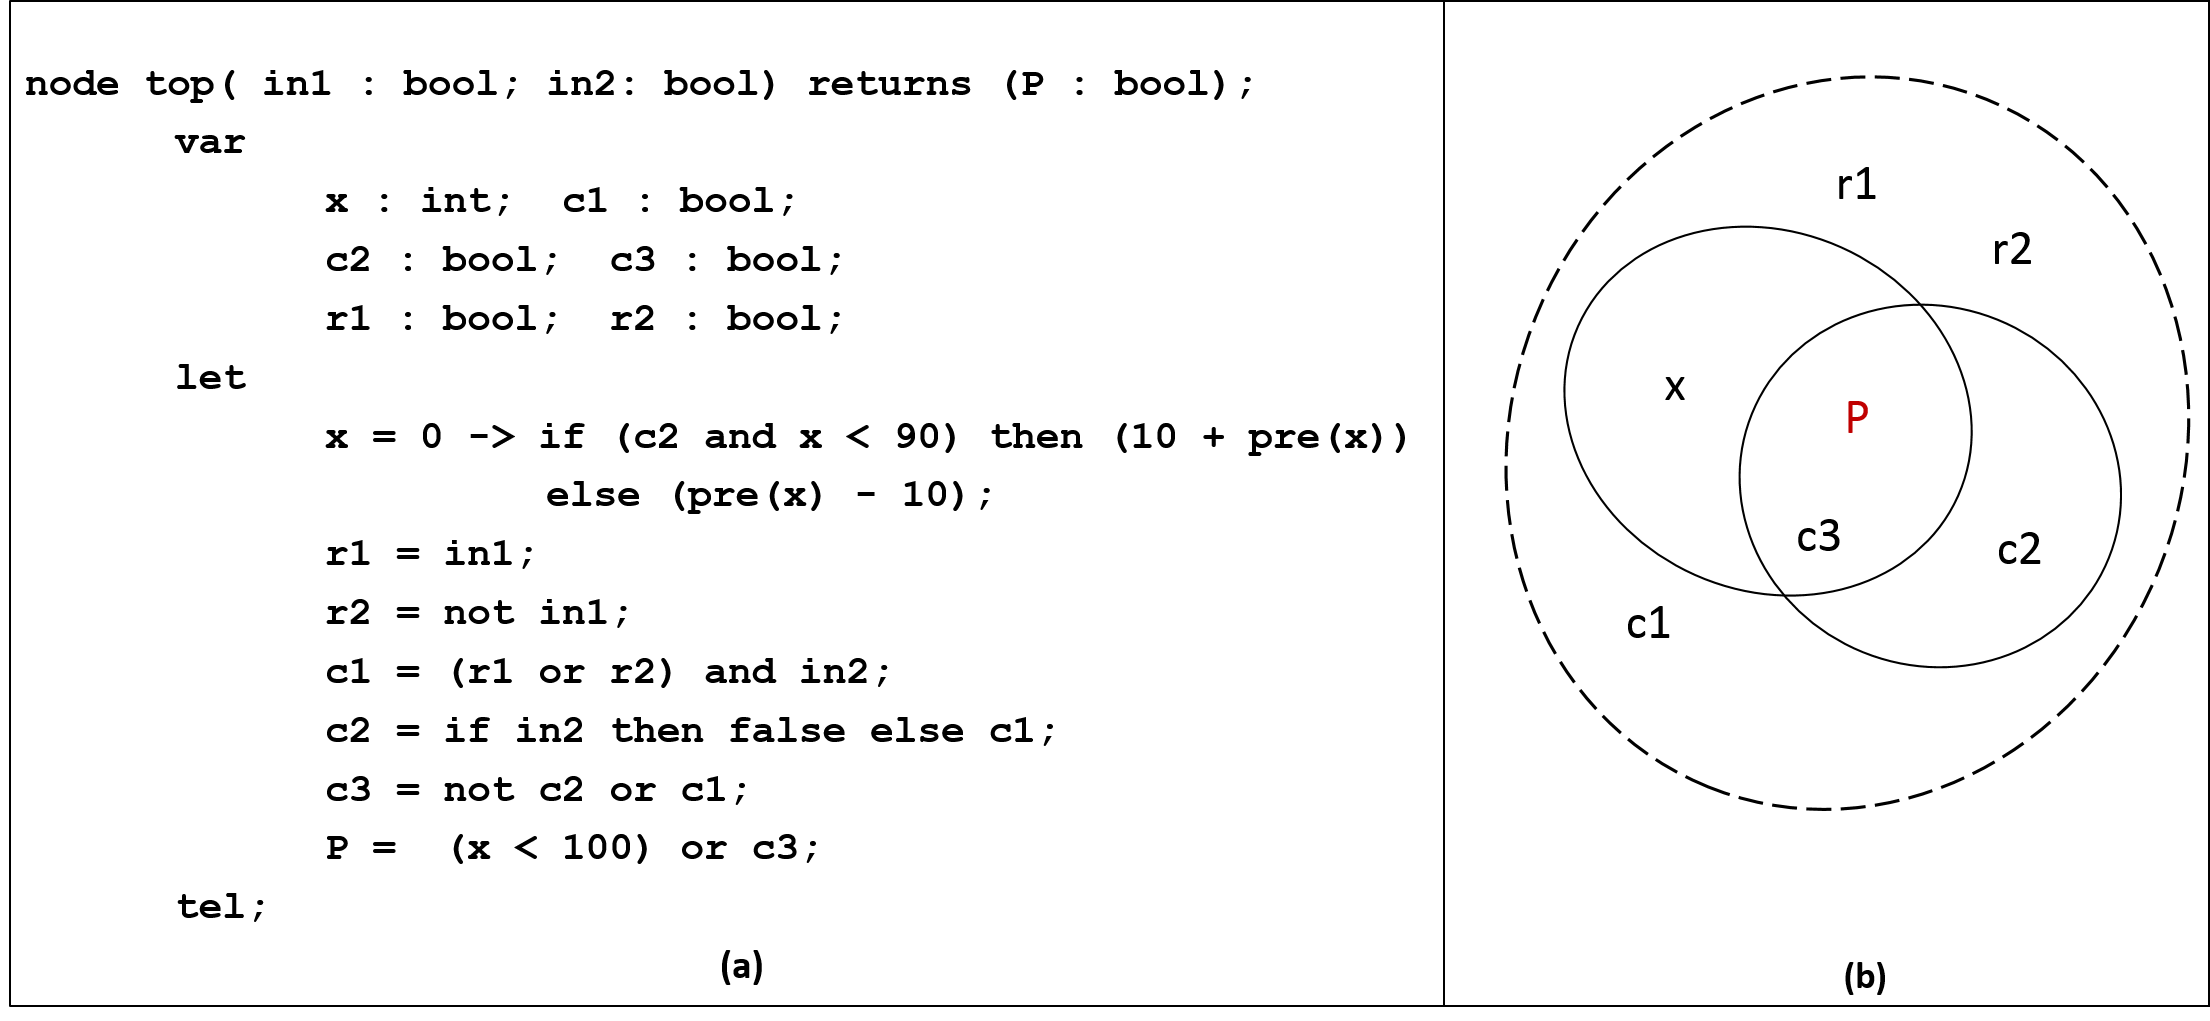
\includegraphics[width=0.8\textwidth]{figs/ex.png}
%\vspace{-0.1in}
%\caption{A Lustre model with property $P$}
%\label{fig:ex}
%\end{center}
%\end{figure*}

%% We put the image here so it shows up side-by-side with fig:ex-after
\begin{figure}[t]
\centering

\includegraphics[width=\columnwidth]{figs/aswcode.png}
%{
%\begin{verbatim}
%node asw(alt1, alt2: int; stat1, stat2 : bool)
%     returns (alarm: bool; doi_on: bool);
%var
%   a1_below, a2_below, below,
%   p1, p2 : bool;
%let
%   a1_below = stat1 and (alt1 < THRESHOLD)  // (1)
%   a2_below = stat2 and (alt2 < THRESHOLD)  // (2)
%   below = a1_below or a2_below             // (3)
%   alarm = not stat1 and not stat2;         // (4)
%   doi_on = if alarm then pre(doi_on)       // (5)
%            else if below then true
%            else false;
%   p1 = a1_below => doi_on;                 // (6)
%   p2 = a2_below => doi_on ;                // (7)
%tel;
%\end{verbatim}
%}
%\vspace{-0.1in}
\caption{Altitude Switch Model with property \small{\texttt{(p1 or p2)}}}
\label{fig:asw}
\end{figure}

We will use a very simple version of an Altitude Switch (ASW) from the avionics domain as a running example (simplified and adapted from~\cite{HCW02:ase-deviation}).
Fig.~\ref{fig:asw} shows the ASW model in the Lustre language.\footnote{Lustre~\cite{Halbwachs91:lustre} is a synchronous dataflow language
used as an input language for various model checkers. A Lustre program runs over discrete
time steps. On each step, the input variables take on some values and
are used to compute values for the output variables on the same step.
In addition, equations may refer to the previous value of a variable
using the \small{{\tt pre}} operator.} In our scenario, the ASW is a hypothetical device that turns power on to another subsystem, the Device of Interest (DOI), when the aircraft descends below a threshold altitude.
For fault tolerance, it is assumed that there are two altimeters that send altitude to the ASW system in terms of input variables \texttt{alt1} and \texttt{alt2}.
It is possible that sensors fail due to different reasons so input variables \texttt{stat1} and \texttt{stat2}, respectively, show the working status of the altimeters \texttt{alt1} and \texttt{alt2}; e.g. when the altimeter \texttt{alt1} is not working, \texttt{stat1} will be \texttt{false}. In the case that both altimeters fail, an ``alarm'' will be triggered (the output \texttt{alarm} will be set to \texttt{true}).
%The notation \texttt{pre(doi\_on))} in equation (7) shows the previous value of \texttt{doi\_on}.
One simple property over this model is that whenever sensors are working and altitude falls below the threshold, output variable \texttt{doi\_on} shall be true. Equations \texttt{p1} and \texttt{p2} show different scenarios under which the DOI might get on. So, we can specify the property in terms of these equations as \texttt{(p1 or p2)}.
In the remainder of the paper, we will use this model for illustration.
